\documentclass[12pt,a4paper]{article}

% Essential packages
\usepackage[utf8]{inputenc}
\usepackage[T1]{fontenc}
\usepackage{graphicx}
\usepackage{amsmath,amssymb}
\usepackage{booktabs}
\usepackage{color}
\usepackage{hyperref}
\usepackage{geometry}
\usepackage{float}

% Hyperlink configuration
\hypersetup{
    colorlinks=true,
    urlcolor=[rgb]{0.2,0.6,0.8},  % Light blue color for URLs
    linkcolor=black,               % Regular internal links remain black
    citecolor=black,               % Citation links remain black
}

% Page geometry
\geometry{margin=2.5cm}

% Document information
\title{Robot Arm Project Report}
\author{Your Name}
\date{\today}

\begin{document}

% Title page
\begin{titlepage}
    \centering
    \vspace*{1cm}
    {\Huge\textbf{Robot Arm Project Report}\par}
    \vspace{2cm}
    {\Large\textit{Project for the introduction to robotics course}\par}
    \vspace{3cm}
    {\Large Luca Sartore\par}
    \vfill
    University of Trento
    \vspace{1cm}
\end{titlepage}

% Table of contents
\tableofcontents
\newpage

% Abstract
\section*{Abstract}
\addcontentsline{toc}{section}{Abstract}
In this report I will describe the project ``robot arm''.
this project consisted in the creation fo a giraffe robot that 
the task of placing the microphone in front of a speaker inside a conference room.
This report will follow the assignment structure, and will therefore
have one section for every of the 8 implementation points in the 
project description that was given to me.
All the source code, as well as the original assignment can be found in the 
github repository \url{https://github.com/lucaSartore/RobotArm}


\section{Step 1 - URDF}
Building the URDF was straightforward enough,
I first focused on the structure and put together one joint at a time,
after that I set up some parameters like the limit and friction of every
joint. Then I focussed on the graphic, and create a visual rapresentation
of the robot using only the basic urdf gemoetric tags sutch as ``box'' and 
``cylinder''; And Finally I insert some mass and inertia values that 
where plausible. The result can be seen in the file \href{https://github.com/lucaSartore/RobotArm/blob/master/src/robot_arm/urdf/arm.urdf}{arm.urdf}

\section {Step 2 - Forward kinematics}
The forward kinematics where computed in the ``classical'' way, using 
progressive transformation matrixes for each joint, where each transformation
matrix depends on q. The code related to this part can be found in the file
\href{https://github.com/lucaSartore/RobotArm/blob/master/src/robot_arm/src/data_processing/direct_kinematics.py}{direct\_kinematics.py}
Here we can see how the joint displacement, as well as the kind of joint are automatically
extracted from the URDF file, using a xml parsing library, and the pydantic framework, then
a transformation matrix is computed using the function ``build\_transf\_matrix\_from\_components''.
Finally all transformation matrixes are multiplied together so to obtain the transformation matrix for the end effector

\section{Step 3 - Simulation}

For the simulation we used the Recursive Newton Euler Algorithm to calculate
the Joint space inertia matrix ($M(q)$) as well as the non linear effects ($h(q,\dot{q})$)
as we have seen in class. Once the forces on the joints where known, they are converted
into joint acceleration (by left-multiplying them with $M(q)^{-1}$) and 
finally they are the acceleration is integrated twice obtain joint velocity and joint position.
The code I described can be found in
\href{https://github.com/lucaSartore/RobotArm/blob/master/src/robot_arm/src/data_processing/dynamics.py}{dynamics.py}

\subsection{Damping, friction and stop force}
The process I dsecirbed so far only considered the forces generated
by gravity, and by the interacgtion between the joints, however in ths simulation
we also included firction, damping and stop forces (forces that are applyed only when a joint
reach the end of his allowed motion range). This where calculated
using the coefficents that where set in the URDF and make the simulation more realistic


\subsection{visualization}

For the visualization the program spawn an rviz process where it constantly 
publish the q position so that the simulation is updated in real time.
To visualize the dynamics yourself you can run one of the following commands:
\begin{itemize}
    \item rosrun robot\_arm main.py test\_dynamics
    \item rosrun robot\_arm main.py test\_dynamics\_with\_initial\_velocity
\end{itemize}


\section{Step 4 - Trajectory}
The trajectory was planned using a fifth degree polynomial that had the constraint of having
to reach an initial and final starting position, as well as needing the
velocity and acceleration (first and second derivative of the polynomial)
to be zero at the start and end.
The variables selected for the trajectory where the X, Y and Z coordinates
as well as the Pitch for orientation. (leaving the other two components of orientation
free).
For the orientation we selected euler angles as they where simple to use, and the singularity
points where really far form the operating range of the robot, making them a non-issue.
The code for the trajectory planning can be seen in
\href{https://github.com/lucaSartore/RobotArm/blob/master/src/robot_arm/src/data_processing/trajectory_planning.py}{trajectory\_planning.py}

\section{Step 5 - Cartesian controller}

The cartesian controller implementation was straightforward, I simply used the 
desired position acceleration, as well as the tracking error, and the tracking error derivative
to calculate the desired v. I then mapped the v in task space into an acceleration in 
joint space, and use the joint space inertia matrix map this to torque.
Finally I linearized of the system by summing the non linear effects.
for the calculation of the non linear effect I fist used the RENA algorithm,
After than realizing that I was computing it twice (one in the dynamics and one in the controller).
Therefore I cashed the result to make the simulation slightly faster.

\begin{align*}
\textcolor{blue}{\mathbf{v}} &= \ddot{\mathbf{p}}^d + K_p (\mathbf{p}^d - \mathbf{p}) + K_d (\dot{\mathbf{p}}^d - \dot{\mathbf{p}}) \\
\textcolor{red}{\ddot{\mathbf{q}}^d} &= J^\# (\textcolor{blue}{\mathbf{v}} - \dot{J} \dot{\mathbf{q}}) \\
\mathbf{u} &= M(\mathbf{q}) \textcolor{red}{\ddot{\mathbf{q}}^d} + c(\mathbf{q}, \dot{\mathbf{q}}) + g(\mathbf{q})
\end{align*}

\section{Step 6 - PD Tuning}

To tune the PD coefficients I started with only the KP, and increase it until the tracking
error become small enough (while being careful not to increase it too much and risking an unstable system).
Once KP was set I started increasing KD until I the value was high enough to make the system critically damped, thus 
avoiding overshooting.

Figure \ref{fig:error_overshoot} and \ref{fig:error_not_overshoot} sows a chart of the absolute value of the
tracking error, In figure \ref{fig:error_overshoot} we can see how the error ``bounces back'' a few time
before reaching zero. In figure \ref{fig:error_not_overshoot} instead we can see how the error monotonically
decreases in the second half part of the chart, this means that the system is not overshooting, thanks 
to the KD being higher.


\begin{figure}[htbp]
    \centering
    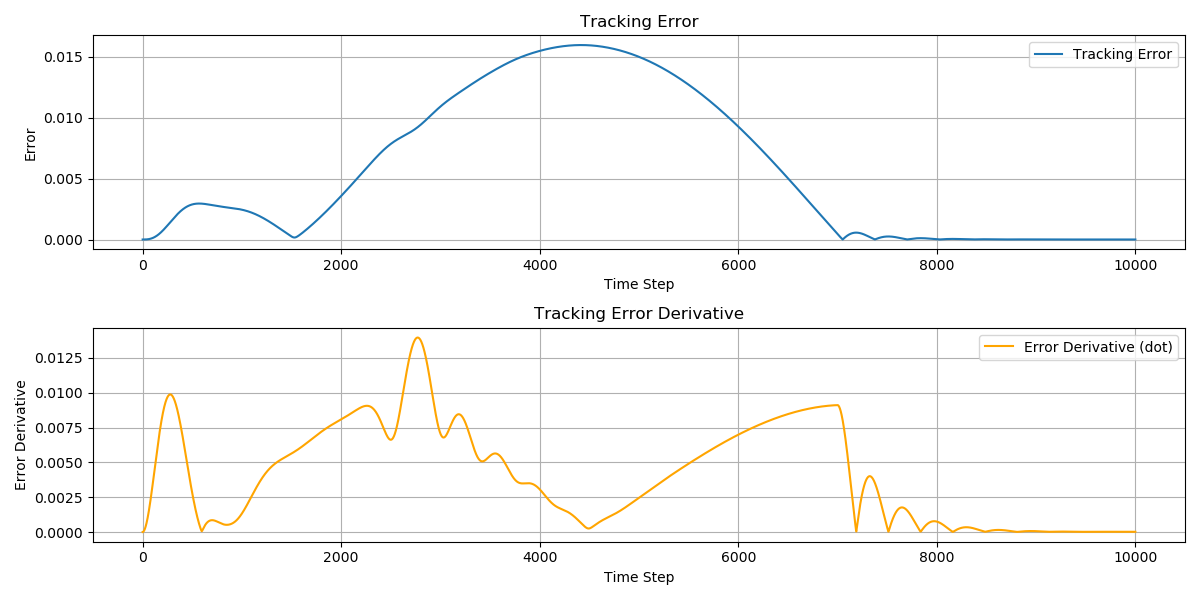
\includegraphics[width=0.7\textwidth]{images/error_chart_overshoot.png}
    \caption{The tracking error overshooting}
    \label{fig:error_overshoot}
\end{figure}


\begin{figure}[htbp]
    \centering
    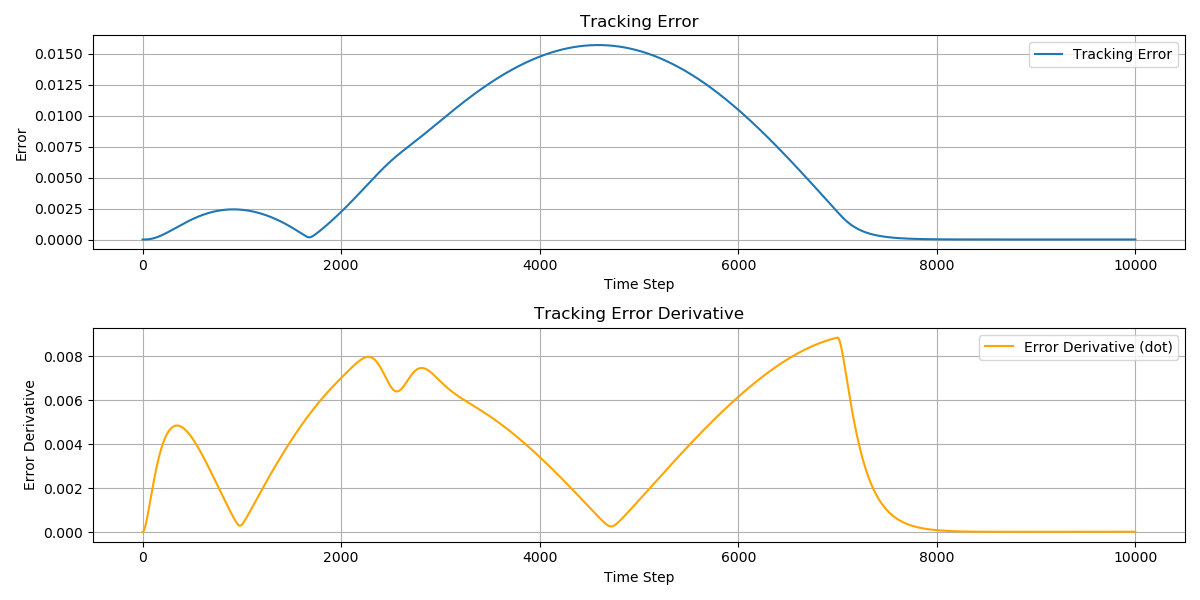
\includegraphics[width=0.7\textwidth]{images/error_chart_no_overshoot.png}
    \caption{The tracking error not overshooting}
    \label{fig:error_not_overshoot}
\end{figure}

\section{Step 7 - Postural task}
Finally since our robot had 5 degrees of freedom, but the task controller only 
specified 4 task-space variables to control, a desired position in joint space was put in
the control loop. The final code can be seen in
\href{https://github.com/lucaSartore/RobotArm/blob/master/src/robot_arm/src/data_processing/controller.py}{controller.py}

\subsection{Selected pose and relative weights}

This postural task can be used guide the robot towards some preferred positions, for example
even to both figure \ref{fig:undesired_pose} and \ref{fig:desired_pose} show poses that are technically
correct, the pose shown in figure \ref{fig:undesired_pose} would be pretty uncomfortable if not dangerous
for the people inside the conference room, in contrast the pose shown in figure \ref{fig:desired_pose}
is much better.

However achieving this result was not as straightforward as one may think. I began by setting a desired
pose where all the q where set to zero, however I quickly realized that not all q have the same importance
In particular the second q (the one controlling the pitch of the longest link) is hte most important, and 
I want it to stay close to zero, to avoid a position similar to the one in figure \ref{fig:undesired_pose}
However other q, like for example the first one (that control the roll of the longest link)
can pretty much have whatever value it wants, and the position will always be decent.

With this observation I implemented a ``weighted'' postural task, where I give more weight
to the joint that I consider more important.

\begin{figure}[H]
    \centering
    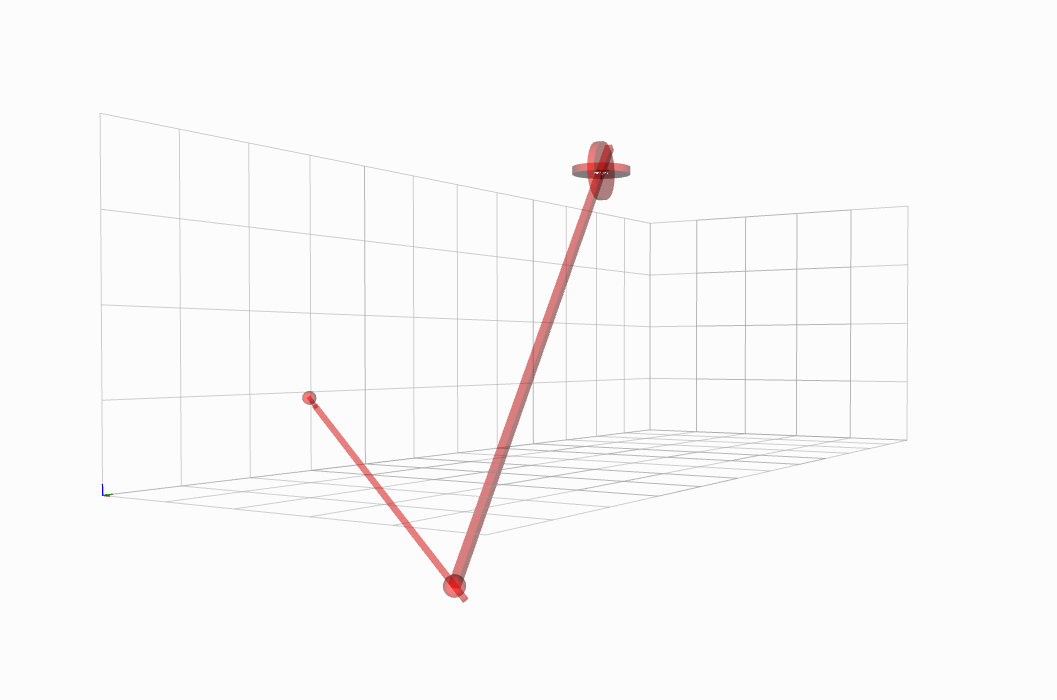
\includegraphics[width=0.7\textwidth]{images/final_position_low.png}
    \caption{An example of an undesired pose}
    \label{fig:undesired_pose}
\end{figure}


\begin{figure}[H]
    \centering
    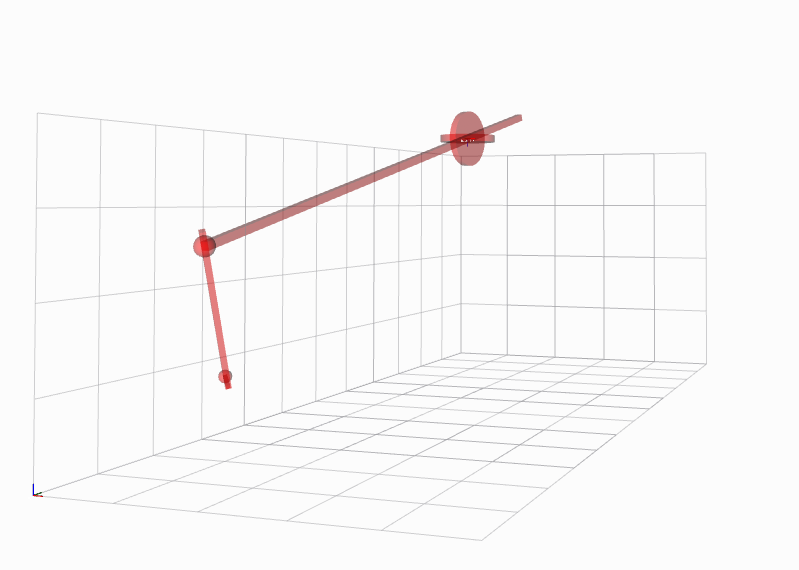
\includegraphics[width=0.7\textwidth]{images/final_positino_high.png}
    \caption{An example of a desired pose}
    \label{fig:desired_pose}
\end{figure}


\section{Step 8 - Simulation}
Finally I put everything together, and ran the simulation with the controller I designed.
The result show the robot reaching the desired position in the 7 second time limit,
and we can see that there is no overshoot.

I uploaded a video of the simulation at this URL: \url{https://www.youtube.com/watch?v=NH_AHPulZkg}. if
if instead you prefer running the simulation yourself you can use the command:
\begin{itemize}
    \item rosrun robot\_arm main.py
\end{itemize}


\end{document}